\chapter{Evaluación experimental y resultados}
\label{chap:evaluacion-resultados}

Este capítulo presenta los resultados obtenidos con los datos experimentales conservados. Se distinguen las métricas registradas durante el entrenamiento del detector, la comparación de una trayectoria automática con anotaciones manuales y el análisis posterior de sus magnitudes de movimiento. Las pruebas controladas del capítulo~\ref{chap:implementacion-pruebas} verifican operaciones e integración; aquí se examina qué información aportan los datos reales y hasta dónde permiten evaluar el sistema desarrollado.

La evidencia cuantitativa de seguimiento se concentra en una trayectoria de referencia parcial. Por tanto, los resultados describen un caso experimental y no una estimación del desempeño sobre todos los microorganismos del video. La reconstrucción posterior de métricas y categorías se identifica como tal para distinguirla de los productos generados durante la ejecución original.

\section{Material experimental y configuración de la prueba}

La prueba analizada corresponde a \texttt{primer\_minuto.mp4}, un video de $1080\times2336$ píxeles, 30 cuadros por segundo y 1800 cuadros, equivalentes a 60 s de imagen. El archivo \texttt{run\_metadata.json} identifica este video y los pesos del modelo adaptado con la versión 1 del dataset. Las versiones y la preparación de los conjuntos de imágenes se describieron en el capítulo~\ref{chap:deteccion}.

El Cuadro~\ref{tab:configuracion-experimental} reúne la configuración conservada. Los umbrales de detección efectivos difieren de los valores predeterminados de la aplicación: la prueba utilizó $0{,}4$ tanto para confianza como para IoU de NMS. Este último parámetro no constituye un umbral de evaluación del seguimiento.

\begin{table}[htbp]
 \centering
 \caption{Configuración documentada de la prueba y del análisis posterior.}
 \label{tab:configuracion-experimental}
 \small
 \begin{tabularx}{\textwidth}{@{}p{0.39\textwidth}X@{}}
  \toprule
  Elemento & Configuración \\
  \midrule
  Video de la prueba & \texttt{primer\_minuto.mp4}. \\
  Modelo & YOLO11x, pesos \texttt{best.pt} de la versión 1. \\
  Confianza e IoU de NMS & $0{,}4$ y $0{,}4$, respectivamente. \\
  Frecuencia de análisis & 30 FPS. \\
  Selección de trayectorias & Al menos 20 observaciones; filtro por cantidad de cuadros. \\
  Clasificación en la corrida original & Desactivada. \\
  Suavizado reconstruido & Media móvil de 20 muestras de rapidez. \\
  Umbrales analíticos & Inactividad: 30 px/s; variación brusca de rapidez: $450$ px/s$^2$; régimen: diferencia de 30 px/s entre ventanas de 50 muestras. \\
  \bottomrule
 \end{tabularx}
\end{table}

Los umbrales analíticos proceden de los metadatos. La ventana de suavizado se reconstruye a partir de la llamada de inspección del notebook, sin un valor alternativo explícito, y del valor predeterminado de la implementación consultada. No figura como campo independiente en los metadatos de aquella corrida. Los valores son operativos y no se presentan como parámetros optimizados experimentalmente.

Se conservaron el archivo de posiciones manuales exportado por Tracker, su normalización en JSON, un CSV de posiciones automáticas y gráficos de trayectoria y movimiento. La referencia normalizada contiene 101 observaciones de un individuo; el CSV automático seleccionado contiene 929 posiciones y se identifica como \texttt{Track\_145.csv}. Los identificadores dependen de cada ejecución y no constituyen identidades biológicas permanentes. El número 2 que aparece en otra salida del notebook no se adopta como identificador equivalente mediante una regla numérica.

El campo de video de la referencia normalizada conserva el nombre \texttt{prueba\_tracker.mp4}. Este nombre corresponde a un archivo distinto de \texttt{primer\_minuto.mp4}; no se utiliza como sinónimo. La identificación del caso se basa en el registro de procesamiento y en la aclaración del autor de las anotaciones de que las pruebas se realizaron sobre \texttt{primer\_minuto}. Se conserva la discrepancia de metadatos para su trazabilidad, sin reinterpretar el nombre original como prueba de identidad entre archivos.

Los metadatos históricos registran Python 3.13.15, pero no las revisiones del código ni todas las versiones de las bibliotecas. El posprocesamiento de este capítulo utiliza los módulos consultados posteriormente, cuyas huellas se conservan junto con los resultados. Esta reconstrucción permite reproducir las operaciones sobre las posiciones disponibles; no certifica que todo el entorno coincida con el utilizado durante la inferencia original.

\section{Resultados registrados del detector}

Se examinaron los archivos de resultados de los dos entrenamientos descritos en el capítulo~\ref{chap:deteccion}, ambos con 100 épocas. El Cuadro~\ref{tab:maximos-detector} resume los máximos individuales de precisión, sensibilidad y mAP. Cada máximo pertenece a su propia época: la fila de una versión no representa una evaluación única con los cuatro valores simultáneos.

\begin{table}[htbp]
 \centering
 \caption{Máximos individuales de las métricas registradas durante el entrenamiento. La época de cada máximo se indica entre paréntesis.}
 \label{tab:maximos-detector}
 \small
 \begin{tabular}{@{}lcccc@{}}
  \toprule
  Dataset & Precisión & Sensibilidad & mAP@0,50 & mAP@0,50:0,95 \\
  \midrule
  Versión 1 & $0{,}98293$ (79) & $0{,}98913$ (83) & $0{,}99216$ (93) & $0{,}76435$ (96) \\
  Versión 2 & $1{,}00000$ (56) & $0{,}95652$ (16) & $0{,}99106$ (58) & $0{,}75651$ (72) \\
  \bottomrule
 \end{tabular}
\end{table}

Para mostrar métricas simultáneas, el Cuadro~\ref{tab:filas-detector} toma la fila completa de la época con mayor mAP@0,50:0,95 de cada entrenamiento. La versión 1 alcanza en esa fila un valor ligeramente superior al de la versión 2. La diferencia describe estos registros; no demuestra una ventaja general de una versión ni permite atribuir causalmente el resultado a los aumentos de datos. No se dispone de repeticiones que cuantifiquen la variabilidad entre entrenamientos y tampoco se ha establecido la independencia temporal de las imágenes de las particiones.

\begin{table}[htbp]
 \centering
 \caption{Métricas simultáneas en la época de mayor mAP@0,50:0,95 de cada entrenamiento.}
 \label{tab:filas-detector}
 \small
 \begin{tabular}{@{}lrcccc@{}}
  \toprule
  Dataset & Época & Precisión & Sensibilidad & mAP@0,50 & mAP@0,50:0,95 \\
  \midrule
  Versión 1 & 96 & $0{,}96178$ & $0{,}97283$ & $0{,}99136$ & $0{,}76435$ \\
  Versión 2 & 72 & $0{,}96921$ & $0{,}94783$ & $0{,}98568$ & $0{,}75651$ \\
  \bottomrule
 \end{tabular}
\end{table}

La Figura~\ref{fig:curvas-detector} muestra la evolución de las dos métricas de mAP. Los valores elevados a IoU $0{,}50$ coexisten con resultados menores al promediar umbrales más exigentes. La diferencia es compatible con la mayor exigencia de localización de las cajas en la segunda métrica; no identifica por sí sola el tipo de error de cada imagen.

\begin{figure}[htbp]
 \centering
 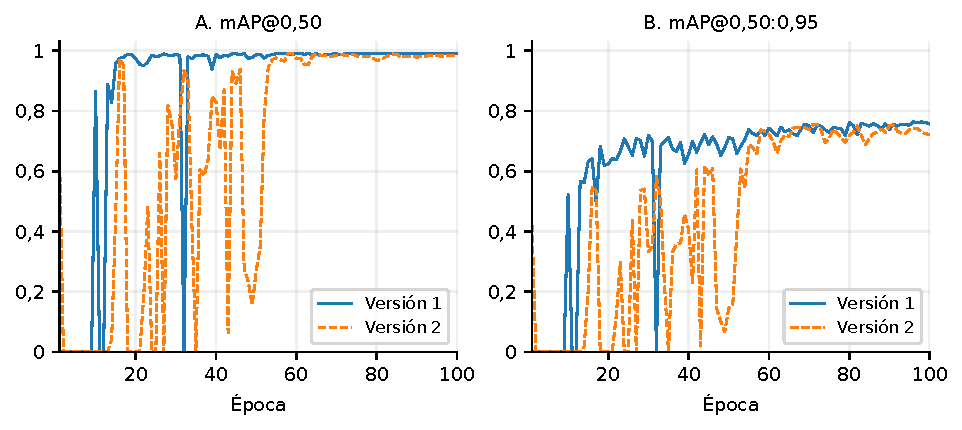
\includegraphics[width=\textwidth]{figures/chapter11/fig11_01_metricas_detector.pdf}
 \caption{Evolución de mAP en los registros de entrenamiento de las dos versiones. Cada punto corresponde a una época. Los registros no constituyen una evaluación adicional del video experimental ni una nueva medición sobre la partición de prueba.}
 \label{fig:curvas-detector}
\end{figure}

Se detectaron valores no numéricos en al menos una pérdida de validación de 11 épocas de la versión 1 y 20 de la versión 2. Las cuatro métricas de detección examinadas contienen valores finitos. Esta incidencia debe conservarse al interpretar el entrenamiento: no se imputaron las pérdidas ni se dedujo su causa a partir del CSV. La información disponible tampoco permite identificar de forma concluyente la época efectiva de \texttt{best.pt}; los cuadros anteriores no se presentan como métricas verificadas de ese archivo de pesos.

\section{Referencia manual y correspondencia temporal}

Las 101 posiciones manuales corresponden a los cuadros 0, 10, 20, hasta 1000. Con 30 FPS, la separación nominal entre anotaciones es de $10/30$ s, aproximadamente $0{,}333$ s. La frecuencia de anotación se distingue de la frecuencia del video. Las filas sin marcación del archivo exportado no se convierten en posiciones ni se rellenan mediante interpolación.

La trayectoria automática abarca los cuadros 0 a 984, con 929 observaciones. La intersección de índices con la referencia contiene 93 cuadros, desde 0 hasta 980. Los cuadros manuales sin posición automática correspondiente son 60, 710, 720, 730, 740, 760, 990 y 1000. Los dos últimos quedan fuera del tramo automático conservado. Las ausencias restantes se encuentran dentro de ese tramo.

La comparación utiliza coincidencia exacta de índice de cuadro. No se asigna una posición automática del cuadro vecino ni se considera un falso positivo cada observación automática sin anotación manual. La referencia es parcial y tiene una resolución temporal menor que el seguimiento. El cociente $93/101$ describe la cobertura de esas anotaciones, no la sensibilidad global del detector ni la exactitud de asociación de identidades.

\section{Alineación del sistema de coordenadas}

Tracker permite definir un origen, una orientación y una escala para transformar posiciones de imagen en coordenadas de análisis \cite{tracker2026}. Por eso, dos recorridos de forma semejante pueden conservar coordenadas numéricas distintas. En el caso estudiado, la coordenada vertical manual aumenta mientras que la coordenada de imagen del modelo disminuye. La semejanza visual se examinó mediante una inversión del sentido de Y y una traslación fijada con el primer par de observaciones.

Las coordenadas iniciales son $(307{,}2;660{,}9)$ para la referencia manual y $(307{,}889282;1667{,}827881)$ para el modelo. Se aplica a todas las anotaciones la transformación
\begin{equation}
 x^{\mathrm{al}}_k=x^{\mathrm{man}}_k,
 \qquad
 y^{\mathrm{al}}_k=C-y^{\mathrm{man}}_k,
 \qquad
 C=y^{\mathrm{mod}}_0+y^{\mathrm{man}}_0
   =2328{,}727881.
 \label{eq:alineacion-tracker}
\end{equation}

El factor de escala permanece en uno; no se rota la trayectoria ni se desplaza X. La constante se obtiene exclusivamente del cuadro 0 y no se reemplaza por la altura del video. En ese cuadro, Y coincide por construcción y persiste una diferencia horizontal aproximada de $0{,}689$ px. Para evaluar los puntos posteriores se excluye el anclaje, de modo que quedan 92 pares entre los cuadros 10 y 980.

Esta operación registra geométricamente la referencia respecto del modelo. No recupera por sí sola la configuración original de Tracker ni establece una equivalencia física con micrómetros. Como utiliza una posición predicha para fijar el origen vertical, los resultados se interpretan como discrepancias después de la alineación, y no como una evaluación independiente de la exactitud absoluta de ese origen.

\section{Comparación de posiciones}

Para cada cuadro común posterior al anclaje se calcula la distancia euclídea entre la posición automática y la manual alineada:
\begin{equation}
 e_k=\sqrt{\bigl(x^{\mathrm{mod}}_k-x^{\mathrm{al}}_k\bigr)^2+
                  \bigl(y^{\mathrm{mod}}_k-y^{\mathrm{al}}_k\bigr)^2}.
 \label{eq:error-posicion-experimental}
\end{equation}
Se resumen su media, mediana, máximo, percentil 95 y raíz del error cuadrático medio, $\mathrm{RMSE}_{p}=\sqrt{\sum_{k=1}^{n}e_k^2/n}$, con $n=92$. No se promedian por separado los errores horizontales y verticales para obtener la media de posición.

\begin{table}[htbp]
 \centering
 \caption{Discrepancia de posición sobre los mismos 92 pares posteriores al anclaje. La comparación directa conserva sistemas de coordenadas incompatibles y se incluye para mostrar el efecto del registro geométrico.}
 \label{tab:errores-posicion}
 \begin{tabular}{@{}lrr@{}}
  \toprule
  Medida (px) & Comparación directa & Referencia alineada \\
  \midrule
  Media & $439{,}120$ & $5{,}328$ \\
  Mediana & $397{,}021$ & $4{,}714$ \\
  RMSE de posición & $507{,}325$ & $6{,}120$ \\
  Percentil 95 & $878{,}154$ & $11{,}338$ \\
  Máximo & $992{,}476$ & $14{,}984$ \\
  \bottomrule
 \end{tabular}
\end{table}

La Figura~\ref{fig:comparacion-tracker} muestra la superposición y las discrepancias por tiempo. De los 92 pares evaluados, 85 tienen una distancia menor o igual que 10 px y los 92 quedan por debajo de 15 px. Estos valores describen la distribución observada; no son tolerancias de aceptación establecidas antes de la prueba. El máximo se encuentra en el cuadro 370, aproximadamente a los $12{,}333$ s.

\begin{figure}[htbp]
 \centering
 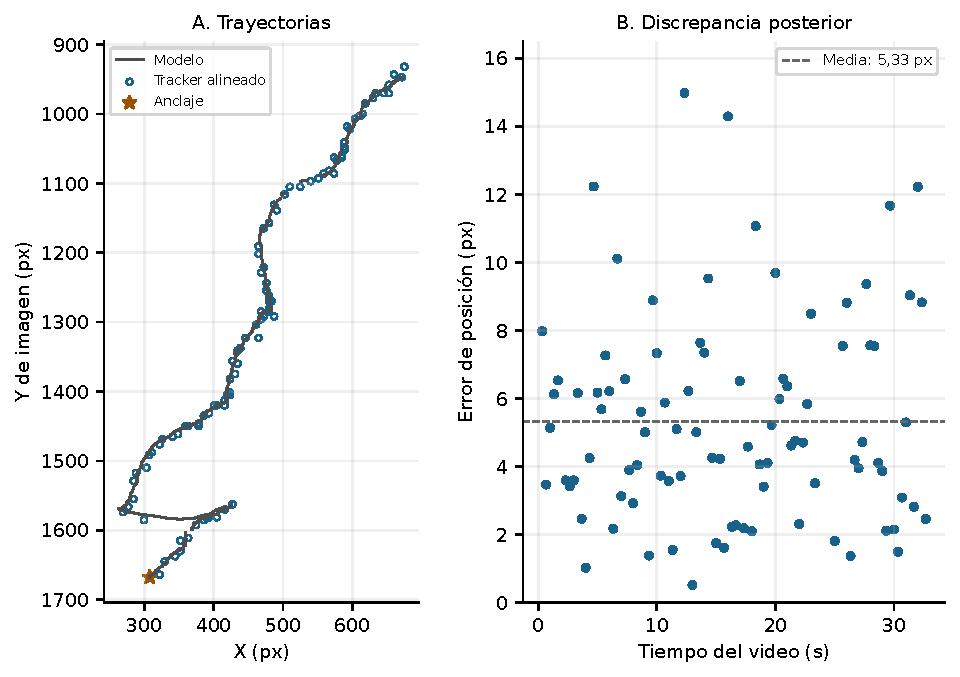
\includegraphics[width=\textwidth]{figures/chapter11/fig11_02_comparacion_trayectorias.pdf}
 \caption{A: posiciones manuales alineadas y trayectoria automática conservada. Los trazos automáticos se interrumpen en los huecos de observación. B: distancia entre posiciones de los mismos cuadros después del anclaje; el cuadro 0 se excluye del resumen. La transformación se mantiene fija para todos los puntos.}
 \label{fig:comparacion-tracker}
\end{figure}

El resultado respalda la similitud geométrica de este par después de la alineación. La comparación directa previa no debe interpretarse como un error de localización de cientos de píxeles atribuible al seguimiento. Aun después del registro persisten diferencias que pueden combinar imprecisión manual, variación del centro de la caja y errores del procesamiento. Una sola anotación por cuadro no permite separar esas contribuciones ni estimar variabilidad entre anotadores.

\section{Continuidad de la trayectoria y observaciones ausentes}

Dentro del intervalo inclusivo de cuadros 0 a 984 hay 985 cuadros posibles y 929 posiciones observadas. La cobertura interna es de aproximadamente $94{,}31$~\%, con 56 cuadros ausentes distribuidos en nueve huecos. El Cuadro~\ref{tab:gaps-experimentales} identifica sus extremos. Los valores se calculan sobre el CSV conservado, sin reconstruir posiciones intermedias.

\begin{table}[htbp]
 \centering
 \caption{Huecos del Track 145. Los extremos son cuadros observados; la cantidad ausente es la diferencia entre extremos menos uno.}
 \label{tab:gaps-experimentales}
 \small
 \begin{tabular}{@{}rrr@{}}
  \toprule
  Último cuadro previo & Primer cuadro posterior & Cuadros ausentes \\
  \midrule
  52 & 54 & 1 \\
  58 & 64 & 5 \\
  694 & 700 & 5 \\
  703 & 722 & 18 \\
  727 & 747 & 19 \\
  759 & 762 & 2 \\
  762 & 764 & 1 \\
  818 & 820 & 1 \\
  821 & 826 & 4 \\
  \midrule
  \multicolumn{2}{@{}l}{Total} & 56 \\
  \bottomrule
 \end{tabular}
\end{table}

Los dos huecos más extensos contienen 18 y 19 cuadros sin observación. La conservación del mismo identificador a ambos lados permite calcular un segmento entre sus extremos, pero no demuestra qué ocurrió durante la ausencia. La pérdida de una posición puede responder a omisión de detección, falta de asociación, oclusión u otras condiciones; el listado de coordenadas no permite asignar una causa visual a cada caso. Tampoco permite contar cambios de identidad ni evaluar cruces de toda la población del video. Esos aspectos quedan pendientes de una revisión específica de imágenes e identidades.

\section{Reconstrucción de las magnitudes de movimiento}

Se aplicaron al CSV las operaciones del capítulo~\ref{chap:analisis-trayectorias}, conservando los índices originales y 30 FPS. El cálculo independiente de distancias, intervalos y cocientes se contrastó con los módulos de rapidez e inspección de la implementación. También coincidieron la media móvil, la clasificación de muestras bajo el umbral de inactividad y las diferencias temporales utilizadas para la variación de rapidez. Esta concordancia verifica la reconstrucción numérica sobre las posiciones disponibles, sin validar nuevamente la inferencia del video.

\begin{table}[htbp]
 \centering
 \caption{Magnitudes reconstruidas del Track 145 completo. La rapidez máxima sin suavizar se distingue del máximo de la media móvil.}
 \label{tab:movimiento-experimental}
 \begin{tabular}{@{}lr@{}}
  \toprule
  Magnitud & Resultado \\
  \midrule
  Tiempo entre primera y última observación & $32{,}8$ s \\
  Distancia acumulada entre observaciones & $1322{,}3331$ px \\
  Desplazamiento neto & $806{,}7973$ px \\
  Rectitud & $0{,}6101$ \\
  Media aritmética de rapideces por segmento & $40{,}2116$ px/s \\
  Rapidez media de trayectoria, distancia/tiempo & $40{,}3150$ px/s \\
  Rapidez máxima por segmento & $403{,}9439$ px/s \\
  Rapidez máxima suavizada & $248{,}2615$ px/s \\
  Muestras suavizadas bajo 30 px/s & $337$ de $909$ \\
  Fracción de muestras suavizadas inactivas & $0{,}3707$ \\
  \bottomrule
 \end{tabular}
\end{table}

La distancia acumulada suma longitudes rectas entre posiciones consecutivas disponibles, incluso al atravesar un hueco. No recupera desplazamientos intermedios no observados. La rapidez por segmento divide cada longitud por su propio intervalo temporal. Por eso, la media de esas rapideces y el cociente entre distancia acumulada y tiempo total son magnitudes diferentes, aunque aquí sus valores sean cercanos.

La media móvil de 20 rapideces produce 909 muestras. De ellas, 337 están estrictamente por debajo de 30 px/s, equivalentes al $37{,}07$~\% de las muestras suavizadas. Este porcentaje no representa directamente una fracción de tiempo ponderada por duración, porque los intervalos no son todos iguales cuando hay huecos. La Figura~\ref{fig:rapidez-experimental} permite examinar la serie original y la suavizada junto con las regiones sin observaciones.

\begin{figure}[htbp]
 \centering
 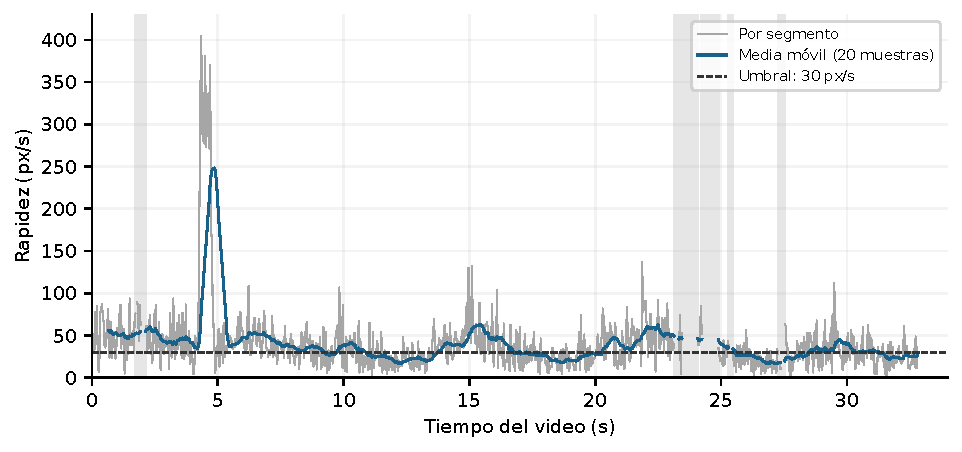
\includegraphics[width=\textwidth]{figures/chapter11/fig11_03_rapidez.pdf}
 \caption{Rapidez por segmento y media móvil de 20 muestras del Track 145. Las regiones grises señalan huecos entre posiciones; las líneas no interpolan esos intervalos. El umbral de 30 px/s se aplica a la serie suavizada para identificar muestras de inactividad.}
 \label{fig:rapidez-experimental}
\end{figure}

Las diferencias temporales de la rapidez suavizada generan 908 valores de variación escalar de rapidez, con extremos de aproximadamente $572{,}53$ y $-553{,}19$ px/s$^2$. Con los umbrales operativos se marcan siete muestras por encima de $450$ px/s$^2$ y cinco por debajo de $-450$ px/s$^2$. La comparación entre medias de ventanas de 50 muestras marca 96 posiciones como posibles cambios de régimen. Las ventanas se solapan: estas cantidades no equivalen a siete, cinco y 96 episodios físicos independientes, ni confirman transiciones biológicas.

\section{Comparación de rapidez con la referencia manual}

La rapidez depende de la resolución temporal con que se observan las posiciones. Para comparar cantidades equivalentes se utilizaron los mismos extremos de los 92 intervalos delimitados por los 93 cuadros comunes. En cada intervalo se calculó la distancia recta entre extremos dividida por el tiempo real, tanto para la referencia alineada como para las posiciones automáticas. En esta comparación no se aplica suavizado ni se suma el recorrido fino del modelo dentro de cada intervalo.

Si $v^{\mathrm{mod}}_j$ y $v^{\mathrm{man}}_j$ son las rapideces del intervalo $j$, se calcularon
\begin{equation}
 \mathrm{MAE}_{v}=\frac{1}{m}\sum_{j=1}^{m}
       \left|v^{\mathrm{mod}}_j-v^{\mathrm{man}}_j\right|,
 \qquad
 \mathrm{RMSE}_{v}=\sqrt{\frac{1}{m}\sum_{j=1}^{m}
       \left(v^{\mathrm{mod}}_j-v^{\mathrm{man}}_j\right)^2},
 \quad m=92.
\end{equation}

El error absoluto medio es de $14{,}0420$ px/s y el RMSE, de $17{,}2047$ px/s. La correlación lineal entre las dos series es de aproximadamente $0{,}8720$. La correlación describe su variación conjunta y no sustituye las medidas de discrepancia. A diferencia de la evaluación de posición, la estimación de los intervalos utiliza también el primer punto como extremo temporal. La inversión y la traslación de Y conservan las distancias entre puntos manuales y, por tanto, sus rapideces; el valor de la constante de alineación no modifica este contraste.

La comparación muestra que la semejanza espacial no implica idéntica precisión al derivar rapidez. Las diferencias entre posiciones de ambos extremos contribuyen al error del desplazamiento y se dividen por un intervalo que suele ser de un tercio de segundo. Además, omitir posiciones intermedias modifica la distancia acumulada: sobre los 93 cuadros comunes, la poligonal automática tiene aproximadamente $1146{,}76$ px, mientras que la referencia manual tiene $1300{,}70$ px. Estos valores corresponden a un tramo y un muestreo diferentes de los 929 puntos del Cuadro~\ref{tab:movimiento-experimental}. No se concluye, a partir de este caso, que la rapidez automática tenga exactitud física suficiente para cualquier uso experimental.

\section{Clasificación posterior del movimiento}

La clasificación estaba desactivada en la corrida original. Para examinar el comportamiento del módulo se aplicó posteriormente el clasificador del capítulo~\ref{chap:clasificacion-movimiento} a las posiciones conservadas, con 30 FPS y sus parámetros predeterminados. Este procedimiento genera una salida nueva de análisis; no se presenta como un archivo de clasificación producido durante aquella inferencia.

El Cuadro~\ref{tab:clasificacion-experimental} muestra las puntuaciones obtenidas sobre la trayectoria completa y sobre las dos secuencias restringidas a los 93 cuadros comunes. Las tres reciben la categoría direccional, aunque sus puntuaciones difieren. El contraste entre la trayectoria completa y su submuestreo muestra que la densidad temporal influye en las características utilizadas por las reglas.

\begin{table}[htbp]
 \centering
 \caption{Puntuaciones del clasificador en el análisis posterior. $Q_D$: direccional; $Q_E$: errático; $Q_C$: circular u oscilatorio. Las puntuaciones son heurísticas, no probabilidades calibradas.}
 \label{tab:clasificacion-experimental}
 \small
 \begin{tabularx}{\textwidth}{@{}Xrccc@{}}
  \toprule
  Secuencia & Puntos & $Q_D$ & $Q_E$ & $Q_C$ \\
  \midrule
  Automática completa & 929 & $0{,}5330$ & $0{,}3497$ & $0{,}5044$ \\
  Automática en cuadros comunes & 93 & $0{,}6186$ & $0{,}1643$ & $0{,}6003$ \\
  Manual alineada en cuadros comunes & 93 & $0{,}5215$ & $0{,}3886$ & $0{,}4706$ \\
  \bottomrule
 \end{tabularx}
\end{table}

En el track completo, la puntuación ganadora supera a la circular u oscilatoria por $0{,}0286$. La asignación es, por tanto, el resultado de la competencia de las reglas y no una afirmación de alta confianza experimental. La rectitud de $0{,}6101$ y la tortuosidad de $0{,}3899$ describen el recorrido observado, pero no identifican un mecanismo físico.

La coincidencia de categoría entre las coordenadas manuales y automáticas aporta una comparación de salidas con el mismo algoritmo. No constituye una validación independiente de la categoría: para medir acierto se requieren etiquetas de referencia asignadas mediante un criterio externo al clasificador. Sin esas etiquetas no se informan exactitud, F1 ni matriz de confusión, ni se considera validada la distinción entre comportamientos direccionales, erráticos y circulares u oscilatorios en la población experimental.

\section{Discusión y alcance de los resultados}

El caso permite vincular una referencia manual parcial con una trayectoria automática y reconstruir sus productos de análisis. La inversión de Y y el anclaje inicial reducen una discrepancia dominada por sistemas de coordenadas incompatibles. Manteniendo fija la transformación, los puntos posteriores conservan una separación media de $5{,}33$ px. Esta evidencia respalda la similitud espacial del par examinado, con las restricciones introducidas por el registro respecto del modelo.

La presencia de huecos no impide obtener métricas con los tiempos reales, pero limita lo que esas métricas representan. La distancia y la rapidez describen conexiones entre observaciones, sin reconstruir el movimiento durante las ausencias. El contraste temporal con Tracker muestra discrepancias de rapidez mayores que las que podría sugerir la superposición visual. Por ello, la validación de posición y la de magnitudes derivadas deben conservarse como evaluaciones diferenciadas.

Los registros de entrenamiento aportan evidencia sobre el detector en las evaluaciones conservadas; no sustituyen una medición de detección sobre el video completo. La referencia de un solo individuo tampoco permite evaluar de forma global conservación de identidad, cruces, oclusiones y fragmentación. La revisión visual específica de esos casos y la disponibilidad de posiciones de otras trayectorias permitirían ampliar la evaluación, sin que la ausencia de ese análisis en este capítulo demuestre ausencia de material experimental.

La clasificación posterior produce resultados inspeccionables, pero su adecuación científica permanece pendiente de comparación con categorías independientes. Los umbrales de inactividad y de cambios de rapidez requieren asimismo una evaluación experimental de su significado, más allá de que el cálculo reproduzca las reglas implementadas.

Las magnitudes se mantienen en px, px/s y px/s$^2$. La alineación con Tracker no determina una escala física. La conversión a micrómetros continúa \textbf{A DEFINIR}, de acuerdo con el alcance establecido en los capítulos metodológicos. Los resultados disponibles permiten documentar la ejecución, su consistencia numérica y una comparación experimental acotada; no justifican todavía generalizaciones a otras condiciones de adquisición o a toda la población de microorganismos.
